\section{Ejercicio \#4: Búsqueda de palíndromos}

Para este ejercicio se busca resolver mediante programación dinámica el problema de obtener la menor cantidad de palíndromos dentro de un string.

\subsection{Supuestos tomados para la resolución del algoritmo}

\begin{itemize}
    \item El algoritmo tiene como entrada un string longitud $n \geq 1$.
    \item Un string de longitud 1 es un palíndromo, por ejemplo, $A$ es un palíndromo.
    \item El acceso a caracteres es $O(1)$ dentro del string.
\end{itemize}

\subsection{Diseño del Algoritmo}

Para la resolución del algoritmo mediante programación dinámica fue necesario analizar en primer lugar la forma que tienen los subproblemas del
problema a resolver, y en segundo la ecuación de recurrencia del mismo.

\subsubsection{Definición del Subproblema}

Sea:
\[
dp[i] = \text{mínima cantidad de palíndromos necesarios para } S[0..i], 
\]

$S[0..i]$ : El string desde la posición $0$ hasta la posición $i$.


\subsubsection{Ecuación de Recurrencia}
\[
dp[i] = \min_{0 \leq j \leq i} \{ dp[j-1] + 1 \mid \text{Si S[j..i] es palíndromo} \}
\]

Condición base:
\[
dp[-1] = 0
\]

Nota: Para una string que va desde $0$ hasta $i$ la ecuación de recurrencia busca obtener la mínima cantidad de palíndromos que hay en todos
los substrings que hay desde $0$ hasta $i$.

\subsubsection{Preprocesamiento de Palíndromos}

Como paso inicial, se define una matriz:

\[
pal[i][j] =
\begin{cases}
True & \text{si } S[i..j] \text{ es palíndromo} \\
False & \text{en caso contrario}
\end{cases}
\]

\[
pal[i][j] = (S[i] = S[j]) \land (j - i \leq 1 \lor pal[i+1][j-1])
\]

Esta permite evaluar si el string que va desde $i$ hasta $j$ es un palíndromo. 

La matriz sirve como estructura de datos auxiliar para el cálculo de la cantidad mínima de palíndromos para cada tamaño  de subproblemas, evitando 
realizar cálculos de forma repetitiva.

\subsubsection{Subestructura Óptima}

La solución óptima para $S[0..i]$ depende de soluciones óptimas de subproblemas $S[0..j-1]$. Esto cumple con la propiedad de la programación dinámica
de resolver un problema a partir del espacio de subproblemas del mismo.

\subsubsection{Subproblemas Superpuestos}

Los valores de $dp[i]$ y $pal[i][j]$ se reutilizan múltiples veces, evitando recomputaciones.

\subsubsection{Memorización}

Se utilizan:
\begin{itemize}
    \item Matriz $pal[n][n]$
    \item Lista $dp[n]$
\end{itemize}

La matriz, tal como se comentó en la sección "Preprocesamiento de Palíndromos" se usa para almacenar que substrings del string original son 
palíndromos. La lista de óptimos almacena la mínima cantidad de palíndromos para todos los substrings de la forma $[0...i]$.

La principal diferencia con la matriz, es que la matriz guarda todas las combinaciones de substring, y la ecuación de recurrencia solo los que van 
de $0$ hasta $i$ (subproblemas del algoritmo).

\subsubsection{Pseudocódigo}

\begin{lstlisting}
def min_palindromos(S):
    n = len(S)

    pal = [[False] * n for _ in range(n)]

    for i in range(n):
        pal[i][i] = True

    for length in range(2, n + 1):
        for i in range(n - length + 1):
            j = i + length - 1

            if S[i] == S[j]:
                if length == 2 or pal[i + 1][j - 1]:
                    pal[i][j] = True

    dp = [0] * n

    for i in range(n):
        if pal[0][i]:
            dp[i] = 1
        else:
            dp[i] = float('inf')
            for j in range(1, i + 1):
                if pal[j][i]:
                    dp[i] = min(dp[i], dp[j - 1] + 1)

    return dp[n - 1]
\end{lstlisting}

\subsection{Seguimiento de ejemplo}

Ejemplo: $S = ABA$

\begin{itemize}
    \item $dp[0] = 1$
    \item $dp[1] = 2$
    \item $dp[2] = 1$
\end{itemize}

Resultado: 1 partición.

\subsection{Complejidad}

Para analizar la complejidad del algoritmo es necesario considerar la complejidad incurrida en cada parte del mismo. Se cuentan con dos partes
principales, el armado de la matriz y el cálculo de los óptimos a partir de la ecuación de recurrencia.

\begin{itemize}
    \item Cálculo de palíndromos: $O(n^2)$
    \item Programación dinámica: $O(n^2)$
\end{itemize}

Complejidad total:
\[
O(n^2)
\]

\subsection{Sets de Datos}

Se utilizaron los siguientes tipos de datos para estudiar al algoritmo:

\begin{itemize}
    \item Mejor caso: cadenas repetidas (ej: AAAA)
    \item Peor caso: caracteres distintos (ej: ABCDEF)
    \item Casos aleatorios con semilla fija
\end{itemize}

\subsection{Tiempos de Ejecución}

Se midieron tiempos utilizando múltiples ejecuciones por cada tamaño de entrada, promediando los resultados para cada tamaño de entrada.

\subsection{Gráfico de los tiempos de ejecución}

Se obtuvo un crecimiento cuadrático en los tiempos de ejecución, consistente con la complejidad teórica.

\begin{figure}[h]
\centering
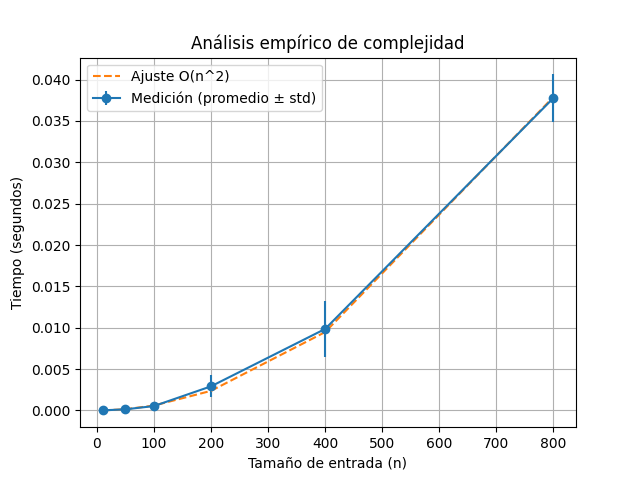
\includegraphics[width=0.8\textwidth]{tex/pd/grafico_tiempos.png}
\caption{Comparación entre tiempos medidos y curva teórica}
\end{figure}

\subsection{Resultados Experimentales}

A continuación se presentan los resultados obtenidos a partir de la ejecución del algoritmo sobre distintos tamaños de entrada:

\begin{center}
\begin{tabular}{|c|c|c|}
\hline
$n$ & Resultado & Tiempo Promedio (s) \\
\hline
10  & 5   & 0.00000941 \\
50  & 13  & 0.00013710  \\
100 & 26  & 0.00053040  \\
200 & 61  & 0.00291414  \\
400 & 127 & 0.00985342  \\
800 & 261 & 0.03777179  \\
\hline
\end{tabular}
\end{center}

\subsection{Análisis de los Resultados}

A partir de los datos obtenidos, se observa que el tiempo de ejecución crece de manera consistente al aumentar el tamaño de la entrada. 
En particular, el crecimiento no es lineal, sino que se acelera a medida que $n$ aumenta, lo cual es indicativo de un comportamiento cuadrático.

Este resultado es coherente con el análisis teórico del algoritmo, cuya complejidad temporal es $O(n^2)$. Si se comparan los tiempos entre 
distintas escalas, se puede notar que al duplicar el tamaño de la entrada, el tiempo de ejecución tiende a multiplicarse 
aproximadamente por un factor cercano a 4, lo cual coincide con el comportamiento esperado de una función cuadrática.

Por ejemplo, al pasar de $n = 200$ a $n = 400$, el tiempo crece de aproximadamente $0.0029$ segundos a $0.0098$ segundos, lo cual 
representa un incremento cercano a cuatro veces. De manera similar, al duplicar nuevamente hasta $n = 800$, el tiempo 
alcanza aproximadamente $0.0377$ segundos, manteniendo la misma tendencia.

\subsection{Comparación con la Curva Teórica}

Al comparar los tiempos medidos con la curva teórica de complejidad $O(n^2)$, se observa que ambos presentan una tendencia similar. 
Esto valida empíricamente el análisis teórico realizado previamente.

Si bien pueden existir pequeñas desviaciones, especialmente en tamaños pequeños donde los costos constantes tienen mayor impacto, 
en general la curva experimental se ajusta adecuadamente al modelo teórico.

\subsection{Conclusión Experimental}

Los resultados obtenidos confirman que el algoritmo presenta un comportamiento cuadrático en la práctica, tal como se había deducido teóricamente. 
Esto demuestra la efectividad del enfoque de programación dinámica utilizado, tanto desde el punto de vista conceptual como en términos de rendimiento.

\subsection{Conclusión}

A lo largo de este trabajo se pudo ver cómo un problema que en principio parece complejo, como probar todas las formas posibles de dividir una cadena, 
puede resolverse de manera eficiente utilizando programación dinámica.

La clave estuvo en cambiar la forma de pensar el problema: en lugar de evaluar todas las particiones posibles, se aprovechó la estructura del 
problema para construir la solución a partir de subproblemas más pequeños. Además, el preprocesamiento de palíndromos permitió 
evitar cálculos repetidos y mejorar significativamente el rendimiento.

En la práctica, los resultados obtenidos muestran que el tiempo de ejecución crece de manera cuadrática con el tamaño de la entrada, 
lo cual coincide con el análisis teórico realizado. Si bien para tamaños pequeños la diferencia no es tan evidente, a medida que crece el tamaño de 
la cadena se observa claramente esta tendencia.

En conclusión, el uso de programación dinámica permitió transformar un problema potencialmente exponencial en uno manejable, 
demostrando la importancia de identificar subestructuras óptimas y reutilizar resultados ya calculados.
